\section{Grafana and PostgreSQL}

To provide a clearer overview of the rover's data, we chose Grafana for real-time visualization.
The incoming data from the rover is stored in a PostgreSQL database with the TimeScaleDB extension, which optimizes the handling of time-series data.

Both Grafana and PostgreSQL run directly on the Raspberry Pi using Docker containers.
However, this setup is flexible since the data is transmitted via MQTT, it can easily be reconfigured to run on a separate server.

The database contains a single table, while different sensors and actuators publish their data to distinct MQTT topics. These topics are used to distinguish between data sources.

The rover’s control unit publishes data to the MQTT topic with the format \texttt{rover/sensor\_name}.
A Python script (\texttt{monitoring/mqtt\_to\_postgres.py}) subscribes to these topics and inserts the incoming data into the database.

The Grafana dashboard (\texttt{monitoring/grafana\_dashboard\_templates/data\_dashboard.json}) is configured to query the database and visualize the data, offering a view of the rover’s state.
The specific topics visualized can be seen in the following image:

\begin{figure}[H]
    \centering
    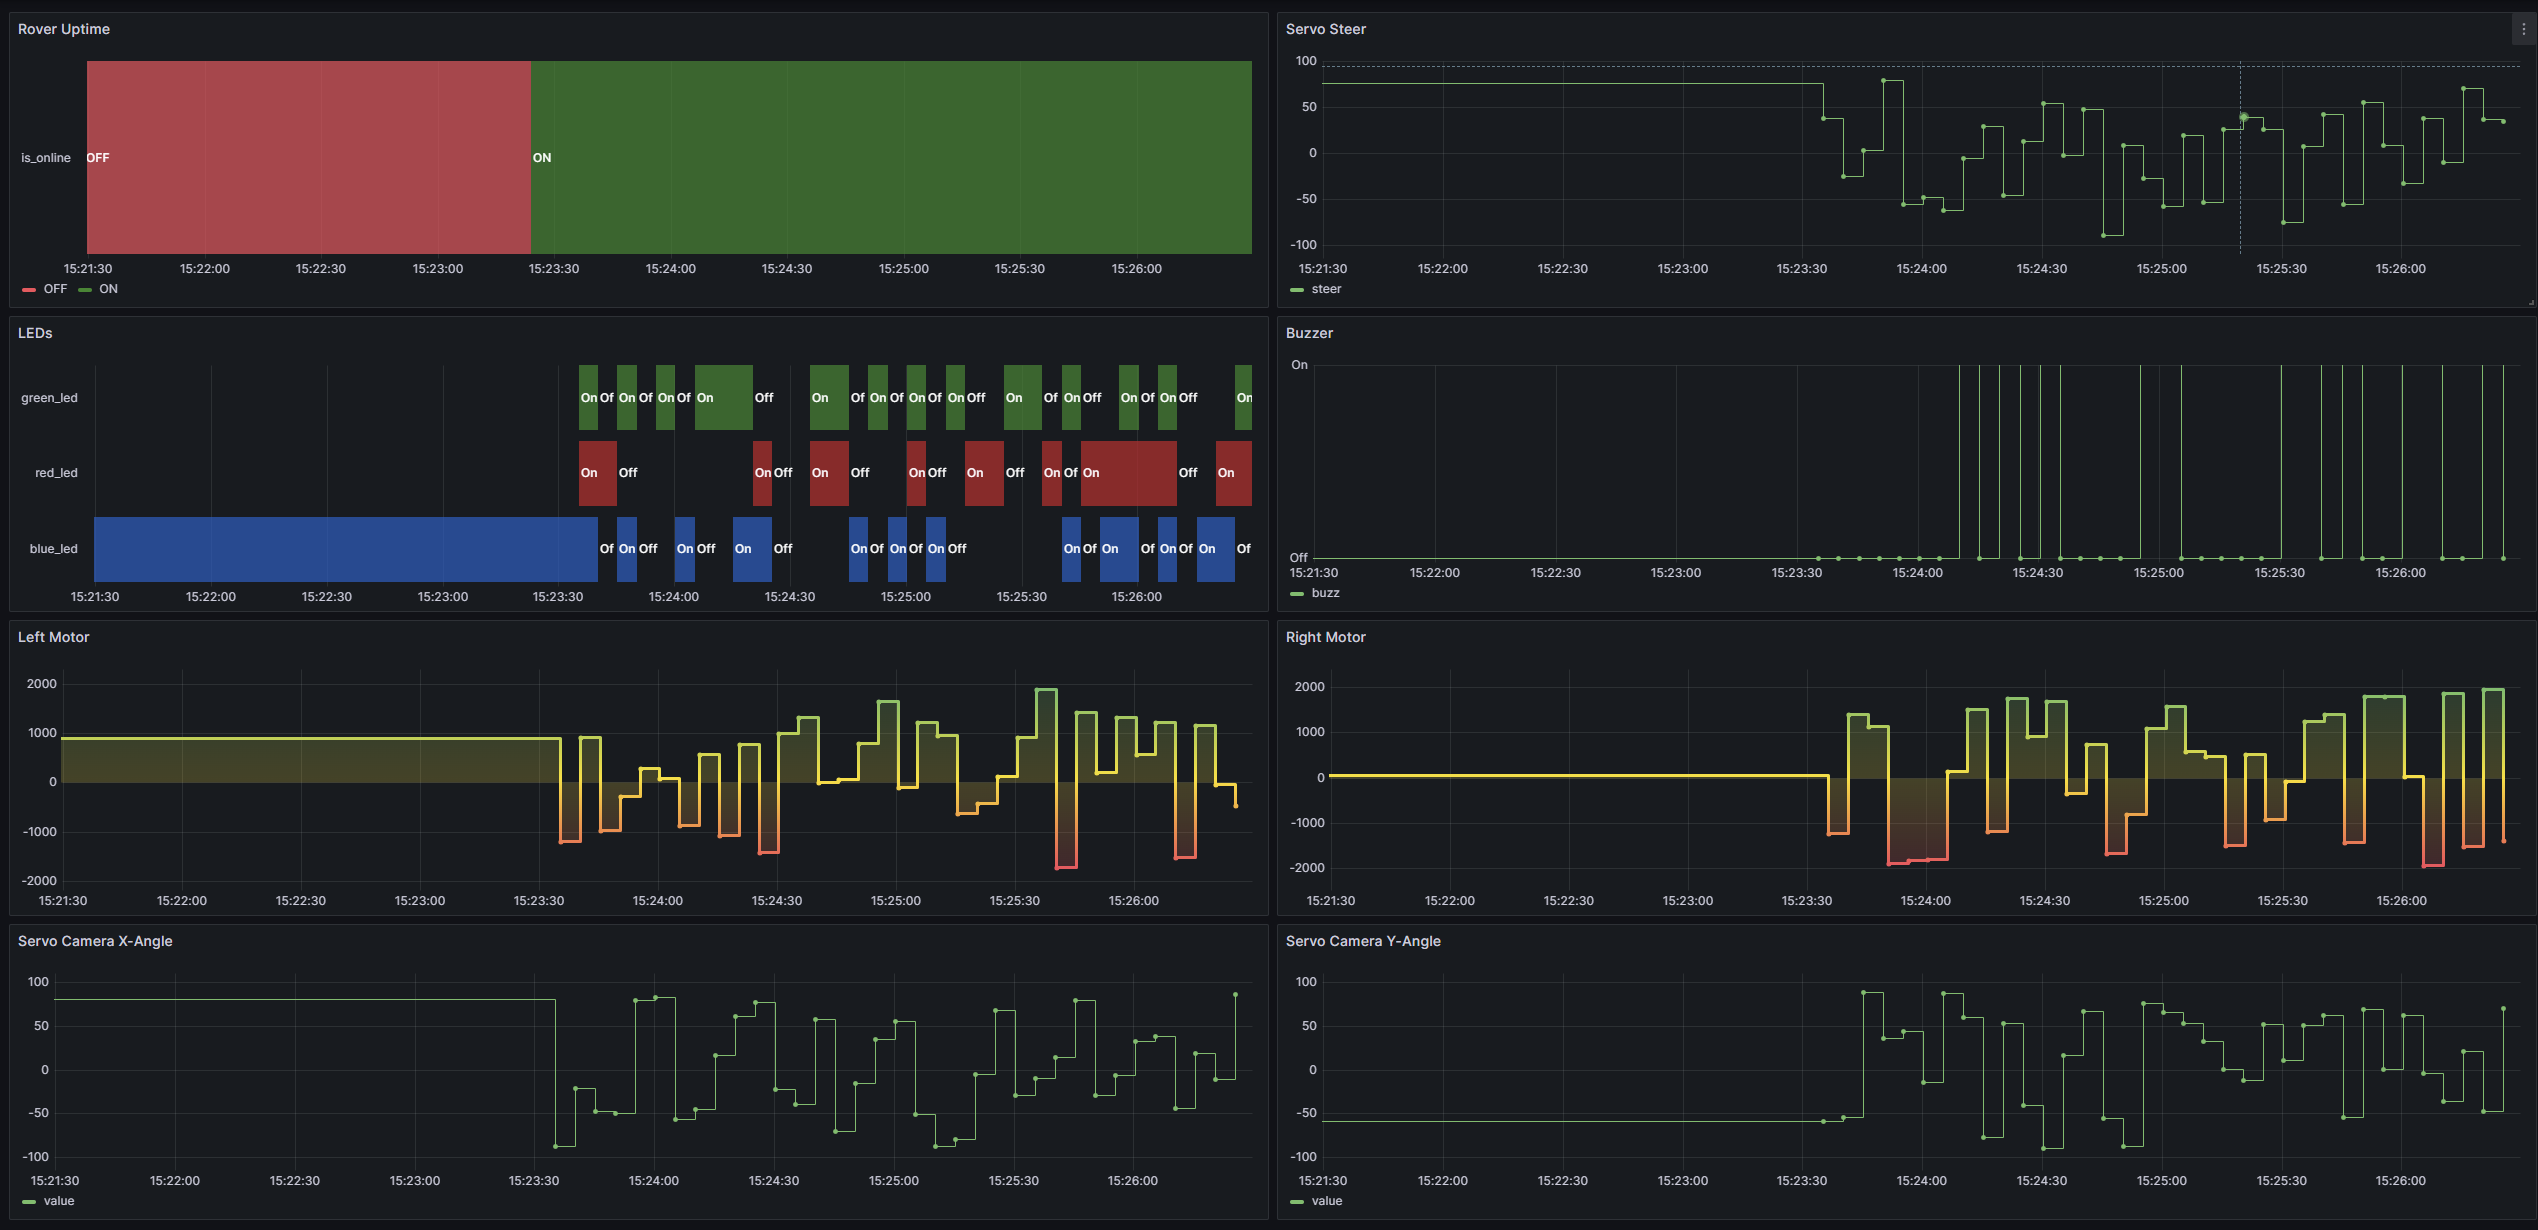
\includegraphics[width=0.95\textwidth]{img/grafana_dashboard}
\end{figure}

